\documentclass[12pt]{article}
\usepackage{graphicx}
\usepackage{caption}
\usepackage{subcaption}
\usepackage{tikz}
\usepackage{venndiagram}
\usepackage{venndiagram}
\usepackage{tcolorbox}
\usepackage{listings}
\usepackage{enumitem}
\usepackage{amsmath}
\usepackage{amssymb}
\usepackage{colortbl}
\usepackage{xcolor}
\usepackage[margin=1cm, top=1.5cm, bottom=1.5cm]{geometry}

\tcbuselibrary{breakable}

\title{\textbf{Gráficas y Juegos: Tarea 04}}
\author{Martínez Méndez Ángel Antonio\\Pinzón Chan José Carlos\\Rendón Ávila Jesús Mateo}
\date{\today}

\begin{document}

\maketitle
\begin{center}
\vspace{3cm}
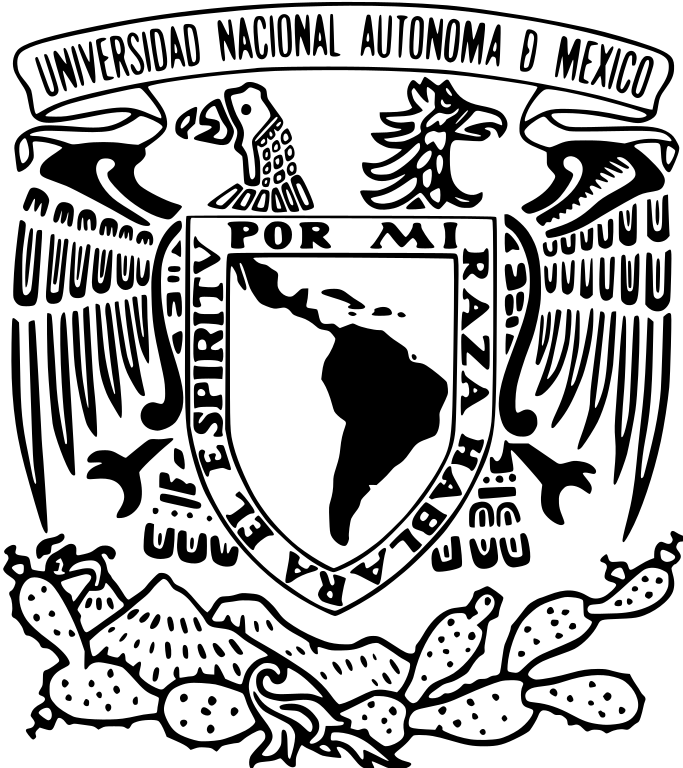
\includegraphics[width=0.195\textwidth]{Escudo.png}
\hspace{0.5cm}
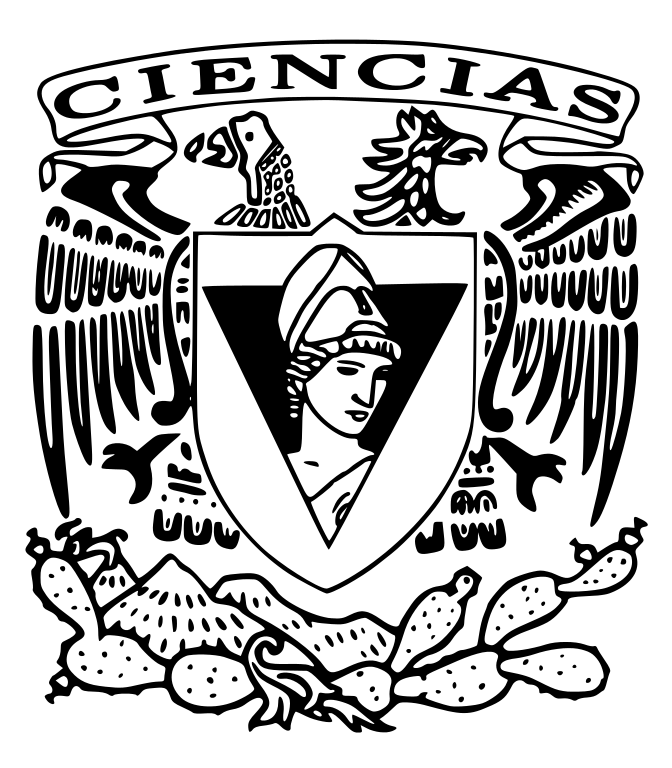
\includegraphics[width=0.2\textwidth]{logo_ciencias.png}
\end{center}
\begin{center}
    \vspace{1cm}
    Universidad Nacional Autónoma de México\\
    Facultad de Ciencias\\
    Profesor: César Hernández Cruz\\
\end{center}

\newpage

%
% Ejercicio 1
%
\textbf{1}. Sea $G$ una gráfica no trivial. Demuestre que $G$ es una trayectoria si 
y sólo si $G$ es un árbol con exactamente dos vértices de grado 1

\begin{tcolorbox}[title=\textbf{Definiciones}, colback=blue!15!white, colframe=black!, breakable]
    $Def$. \textbf{Trayectoria}: Un camino que no repite vertices.
\end{tcolorbox}

{\color{blue} [$\Rightarrow]$} Sea $G$ una trayectoria no trivial.\\

Como la gráfica es no trivial; significa que, al menos, tiene dos vertices $u,v \in V_G$ adyacentes por una 
arista $uv \in E_G$, donde ambos $d(v)=1$, $d(u)=1$. Y como se trata de una trayectoria; entonces no tiene lazos, es aciclica, 
conexa y su número de aristas corresponde a $|E| = |V|-1$.\\

Notemos que al tratarse de un árbol, si tuvieramos el caso en que la gráfica $|V_G| \geq 3$ y grado máximo $\Delta < 3$ entonces 
los extremos de nuestros vertices siempre van a ser $d(v_0)=1$, $d(u_n)=1$. Y todo vertice que este entre estos dos 
$v_0 \leq v_j \leq u_{j-1} \leq u_n$ donde $j \in \{1, 2, 3, j-1...\}$ van a tener grado $d(v_j)$, $d(u_j) = 2$.\\

El caso donde tenemos grado máximo $\Delta = 3$ no se da, porque no podríamos asegurar que la gráfica sea una 
trayectoria, ya que se ramifica la gráfica.\\

De tal modo que si nuestra gráfica tiene vertices con $\Delta = 2$ entonces los extremos de nuestro árbol tendrán $d(v)=1$, $d(u)=1$.\\

{\color{blue} [$\Leftarrow]$} Sea $G$ un árbol con exactamente dos vértices de grado 1.\\

Sabemos que para un árbol no trivial, siempre va a existir un vértice que lo conforme que será de grado máximo 
$\Delta = 2$ y sus hojas de grado 1.\\

Para el caso en en el que tenemos $|V_G| \geq 3$ podemos construir un camino $P$ que tiene como extremos a las hojas 
$x, y \in V_G$ y a través de el podemos recorrer todo el árbol de forma única.\\

Suponiendo que existe un vértice extra que sale de algún vértice intermedio de $x, y$, digamos $w$, entonces se trataria de una nueva hoja con $d(w) = 1$, lo cual contradice 
nuestra hipotesis, pues el árbol que construimos solo admite dos vértices de grado 1.\\

Por lo que, este $xy$-camino, en realidad se trata de una trayectoria con sus extremos $d(x)=1$, $d(y)=1$

\hfill $\Box$

\vspace{1cm}

%
% Ejercicio 2
%
\textbf{2}.
\begin{enumerate}[label = $\alph*)$]

    \item Demuestre que cada árbol con grado máximo $\Delta >$ 1 tiene al menos $\Delta$  hojas.\\
    
    \begin{tcolorbox}[title=\textbf{Hipótesis}, colback=red!15!white, colframe=black!]
        
    Un árbol con grado máximo $\Delta >$ 1.
     
    \end{tcolorbox}
        
    \begin{tcolorbox}[title=\textbf{Definiciones}, colback=blue!15!white, colframe=black!]
         $Def$. El grado máximo de una gráfica G, es el grado máximo de todos sus vértices.
    \end{tcolorbox}
     
    \item Construya, para cada eleccion de $n$ y $\Delta$, con 2 $\leq$ $\Delta < n$, un árbol de orden $n$ con exactamente $\Delta$ hojas.
    \end{enumerate}
    
    \textbf{Demostración inciso a):}\\
    
    Sea $G$ un árbol con grado máximo $\Delta = k$ donde $k >$ 1.\\
    
    Por hipótesis para algun vértices $u \in V_G$ existen $k$ aristas incidentes en él. Sea $uv$ alguna de las $k-aristas$. Si tomamos una trayectoria máxima  $W$ = \{$u, uv, v, ... , v_i$\} se cumple que es única (ya que G es un árbol) y además no repite vértices (por la definición de trayectoria). \\
    
    Como $W$ es única  y no repite vértices, entonces el último vértice ($v_i$) tiene grado 1, pues en caso contrario la trayectoria no es máxima y/o bien repite vértices. De este modo se concluye que $v_i$ es una hoja.\\
    
    Como existen $k$ aristas distintas que inciden en $u$, entonces en $G$ existen por lo menos  $k$ $uv_i-trayectorias$ de longitud máxima. Por lo tanto, $G$ tiene cuando menos $k = \Delta$ hojas.\\
    
    
    \begin{figure}[h!]
        \begin{subfigure} {0.5\textwidth}
                    \centering
                    \begin{tikzpicture}[scale=1.5]
                        \node (a) at (0,0) [circle,fill,inner sep=1.5pt, color = blue] {};
                        \node [anchor=west, color = blue] at (0,0.1) {$\tiny u $};
                        \node (b) at (1,0) [circle,fill,inner sep=1.5pt] {};
                        \node (c) at (-1,0) [circle,fill,inner sep=1.5pt] {};
                        \node (d) at (2,0.5) [circle,fill,inner sep=1.5pt] {};
                        \node (e) at (-2,-0.5) [circle,fill,inner sep=1.5pt] {};
                        \node (f) at (0.3,-1) [circle,fill,inner sep=1.5pt] {};
                        \node (g) at (0,1) [circle,fill,inner sep=1.5pt, color = blue] {};
                        \node [anchor=south, color = blue] at (0,1.1) {$\tiny v $};
                        \node (h) at (-0.5,2) [circle,fill,inner sep=1.5pt] {};
                        \node (i) at (0.5,2) [circle,fill,inner sep=1.5pt] {};
                        \node (k) at (0.5,3) [circle,fill,inner sep=1.5pt] {};
    
                    \draw [blue] (a) -- (g);
                        \draw (a) -- (b) (b) -- (d) (a) -- (c) (c) -- (e);
                        \draw (a) -- (f) (g) -- (h) (g) -- (i);
                        \draw (i) -- (k) ;
    
    
                    \end{tikzpicture}
                    \caption{\scriptsize Ejemplo de la arista $uv$ (Note que $u$ es el vértice con mayor grado).}
                \end{subfigure}
                \begin{subfigure} {0.5\textwidth}
                    \centering
                    \begin{tikzpicture}[scale=1.5]
                        \node (a) at (0,0) [circle,fill,inner sep=1.5pt, color = red] {};
                        \node [anchor=west, color = red] at (0,0.1) {$\tiny u $};
                        \node (b) at (1,0) [circle,fill,inner sep=1.5pt] {};
                        \node (c) at (-1,0) [circle,fill,inner sep=1.5pt] {};
                        \node (d) at (2,0.5) [circle,fill,inner sep=1.5pt] {};
                        \node (e) at (-2,-0.5) [circle,fill,inner sep=1.5pt] {};
                        \node (f) at (0.3,-1) [circle,fill,inner sep=1.5pt] {};
                        \node (g) at (0,1) [circle,fill,inner sep=1.5pt, color = red] {};
                        \node [anchor=south, color = red] at (0,1.1) {$\tiny v $};
                        \node (h) at (-0.5,2) [circle,fill,inner sep=1.5pt,] {};
                        \node (i) at (0.5,2) [circle,fill,inner sep=1.5pt,color = red] {};
                        \node (k) at (0.5,3) [circle,fill,inner sep=1.5pt,color = red] {};
                        \node [anchor=west, color = red] at (0.6,3) {$\tiny v_i $};
    
                    \draw [red] (a) -- (g) (g) -- (i) (i) -- (k) ;
                        \draw (a) -- (b) (b) -- (d) (a) -- (c) (c) -- (e);
                        \draw (a) -- (f) (g) -- (h) ;
    
    
                    \end{tikzpicture}
                    \caption{\scriptsize Ejemplo de trayectoria máxima que contiene a $uv$ ($v_i$ es una hoja).}
                \end{subfigure}
           
    \end{figure}
    En los ejemplos de arriba queda claro el porque del "al menos", pues pueden existir otras trayectorias  que también contengan a la arista $uv$ y que a partir de cierto vértice no se encuentren contenidas en la trayectoria máxima.
    
    
    \textbf{Inciso b):}\\
    
    Por la demostración anterior sabemos que al construir un árbol con grado máximo $\Delta$ exsiten al menos $\Delta$ hojas, sin embargo, en esta ocasión queremos asegurarnos que el número exacto de hojas sea $\Delta$.\\ 
    
    La característica principal que cumple una hoja es que es un vértice con grado 1. Entonces si queremos tener $\Delta$ hojas, necesitamos  $\Delta$ vértices con grado 1. Si queremos seguir cumpliendo con que la gráfica sea conexa entonces dichos vértices deben estar conectados (no necesariamente de forma directa) por un vértice común, dicho vértice entonces tendrá grado $\Delta$. Hasta este momento hemos contemplado $\Delta$ + 1 vértices, pero si $n > \Delta + 1$, entonces, ¿qué hacemos con los vértices restantes?\\
    
    La respuesta es bastante sencilla, los vértices restantes deben tener grado 2, pues en ese caso tienen un vértice anterior y un vértice siguiente, es decir, forman una trayectoria y aquello nos permite tener vértices de grado 1 al final. Como tenemos $n$ vértices, y $\Delta$ son de grado 1 y uno mas de grado $\Delta$, esto implica que el número de vértices restantes (de grado 2) es igual a $n - \Delta - 1$.\\
    
    Finalmente, para construir un árbol $T$ con $\Delta$ hojas, donde $2 \leq \Delta < n$, tiene que suceder que su sucesión de grados tenga la siguiente forma:
    \begin{center}
    $ d_T = (\Delta , 2_1 , 2_2 , ... , 2_{(n - \Delta - 1)} , 1_1 , 1_2 ,..., 1_\Delta)$\\
    \end{center}
    
    Vamos a probar nuestra construccion con algunos ejemplos.\\
    \begin{enumerate}
    
        \item $\Delta$ = 2 y $n$ = 3.
        
        Note que debe suceder lo siguiente:\\
        
        \begin{list}{•}{ }
        \item Un vértice debe tener grado $\Delta$.
        
        \item Deben existir 3 -2 -1 = 0 vértices de grado 2.
        
        \item Deben existir 2 vértices con grado 1.
        \end{list}
        La sucesión de grados de nuestro árbol $T'$ es: $d_{T'} = (2 , 1 , 1)$\\
        
        \vspace{0.5cm}
        \begin{figure}[h!]
             \captionsetup[figure]{font=small}
             \centering
                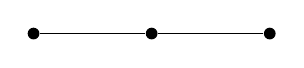
\begin{tikzpicture}[scale=1.5]
                        \node (a) at (0,0) [circle,fill,inner sep=1.5pt] {};
                        \node (b) at (1,0) [circle,fill,inner sep=1.5pt] {};
                        \node (c) at (-1,0) [circle,fill,inner sep=1.5pt] {};
    
                    \draw (a) -- (b) (a) -- (c);
                \end{tikzpicture}
                \caption{Gráfica de $T'$.}
        \end{figure}
        
        \item $\Delta$ = 4 y $n$ = 7.
        
        Note que debe suceder lo siguiente:\\
        
        \begin{list}{•}{ }
        \item Un vértice debe tener grado $\Delta$.
        
        \item Deben existir 7 -4 -1 = 2 vértices de grado 2.
        
        \item Deben existir 4 vértices con grado 1.
        \end{list}
        La sucesión de grados de nuestro árbol $T''$ es: $d_{T''} = (4 , 2 , 2 , 1 , 1 , 1 , 1)$\\
    
        \begin{figure}[h!]
             \captionsetup[figure]{font=small}
             \centering
                \begin{tikzpicture}[scale=1.5]
                        \node (a) at (0,0) [circle,fill,inner sep=1.5pt] {};
                        \node (b) at (1,0) [circle,fill,inner sep=1.5pt] {};
                        \node (c) at (-1,0) [circle,fill,inner sep=1.5pt] {};
                        \node (d) at (-2,0) [circle,fill,inner sep=1.5pt] {};
                        \node (e) at (2,0) [circle,fill,inner sep=1.5pt] {};
                        \node (f) at (0,1) [circle,fill,inner sep=1.5pt] {};
                        \node (g) at (-0,-1) [circle,fill,inner sep=1.5pt] {};
    
                    \draw (a) -- (b) (a) -- (c) (b) -- (e) (c) -- (d) (a) -- (f) (a) -- (g);
                \end{tikzpicture}
                \caption{Gráfica de $T''$.}
        \end{figure}
    
    \end{enumerate}

\vspace{1cm}
%
% Ejercicio 3
%
\textbf{3}.Un centro de una gráfica es un vértice $u$ tal que $max_{u\in V}d(u,v)$ es mínima. Demuestre que un árbol tiene exactamente un centro o  2 centros adyacentes. 

\begin{tcolorbox}[title=\textbf{Hipotesis}, colback=red!15!white, colframe=black!]
    Sea $T$ un árbol. 
\end{tcolorbox}
\begin{tcolorbox}[title=\textbf{Definiciones}, colback=blue!15!white, colframe=black!]
        $max_{u\in V}d(u,v)$ se puede interpretar como que la excentricidad de $u$ es la más pequeña de todas las excentricidades de la gráfica.
\end{tcolorbox}

Como $T$ es un árbol, la distancia entre cualesquiera $u,v \in_{V_T}$ es la longitud de su $uv-trayectoria$.\\

Sea la excentricidad de un $v\in_{V_T}$ igual a la longitud de la trayectoria $W$ = \{$v,...,v_k$\} entonces $v_k$ es una hoja (en otro caso no sería la excentricidad de $v$ o bien no sería una trayectoria). En consecuencia las excentricidades de los vértices en $T$ corresponden a su mayor distancia a alguna hoja.\\

El centro de un árbol es el vértice cuya excentricidad es mínima (su mayor distancia a alguna hoja es mínima, en comparación con las mayores distancias de otros vértices hacia hojas).\\ 

Como $T$ es conexa cualquier vértice puede alcanzar a cualquier hoja. Si tomamos la trayectoria máxima $S$ de $T$, $S$ = \{$v_1,...,v_i,...,v_n,...,v_j,...,v_k$\} (donde $i < n$ y $j >n$) , dicha trayectoria tiene hojas como elementos extremos. Como $S$ es la trayectoria máxima podemos asegurar que $v_1$ y $v_k$ son los vértices más "lejanos" entre si. De forma más general, son los vértices más "lejanos" en $T$.\\

Si la longitud de $S$ es impar, entonces podemos ubicar $v_n \in S$ tal que se encuentre justo en la mitad de la trayectoria $S$. Como resultado su máxima distancia (excentricidad) corresponde a la longitud de $d(v_n, v_1)$ = $d(v_n, v_k)$. Esta va a ser menor que la longitud de $d(v_j,v_1)$ y la longitud de $d(v_i,v_k)$ para todo $v_i,v_j$ (evidentemente distintos de los extremos y de $v_n$). Como la longitud de estas distancias corresponde a la excentricidad de los vértices, entonces la excentricidad de $v_n$ es menor que la excentricidad de todo $u \in {V_T}$. Por lo tanto $v_n$ es centro y además es único.\\

Si la longitud de $S$ es par, entonces podemos ubicar $v_m,v_{m+1} \in S$, ($m$ = longitud de $S$ entre dos) tal que se encuentren en la mitad de la trayectoria $S$. Como resultado su máxima distancia (excentricidad) corresponde a la longitud de $d(v_m, v_k)$ y de $d(v_{m+1}, v_1)$ respectivamente. Sea $i < m$ y $j > m + 1$, entonces la longitud de  $d(v_m,v_k) < d(v_i,v_k)$ y la longitud de $d(v_{m+1},v_1) < d(v_j,v_1)$ para todo $v_i,v_j$ (evidentemente distintos de los extremos y de $v_m,v_{m+1}$). Como la longitud de estas distancias corresponde a la excentricidad de los vértices, entonces las excentricidades de $v_m,v_{m=1}$ son menores que las excentricidades de todo $u \in {V_T}$ ($u \neq v_m,v_{m+1}$)  . Por lo tanto $T$ tiene exactamente dos centros ($v_m,v_{m=1}$) y además son adyacentes. Queda implícito que la excentricidad de $v_m$ es igual a la excentricidad de $v_{m+1}$.


\vspace{1cm}
%
% Ejercicio 4
%
\textbf{4}. Demuestre o brinde un contraejemplo: Toda gráfica con menos aristas que vértices tiene una ocmponente que es un árbol.

\begin{tcolorbox}[title=\textbf{Hipotesis}, colback=red!15!white, colframe=black!, breakable]
	$|E(G)| < |V(G)|$ 
\end{tcolorbox}

\begin{tcolorbox}[title=\textbf{Definiciones}, colback=blue!15!white, colframe=black!, breakable]
    $Def$. Una gráfica $G$ es un árbol si y sólo si $G$ es conexa y no contiene ciclos.
\end{tcolorbox}

$Dem$. Por casos.\\

Sea $G$ una gráfica que, por hipotesis $|E(G)| < |V(G)|$, entonces tendremos que $G$ puede ser conexa o inconexa. Así tenemos dos casos:
\begin{enumerate}
    \item $G$ es conexa
    \item $G$ no es conexa
\end{enumerate}

$Caso$ 1. como $G$ es conexa entonces existe una trayectoria entre cualesqueira dos vértices $u,v \in V(G)$, por hipotesis sabemos que 
esta trayectoria es única pues $G$ no contiene ciclos, es decir $G$ es un árbol.\\

$Caso$ 2. Como $G$ no es conexa, entonces $G$ tiene 2 o más componentes, de nuevo por hipotesis, al menos una de 
estas gráficas componentes de $G$, llamemosle $T$, tendrá que satisfacer la condición de la hipotesis, $i.e$ $|E(T)| < |V(T)|$,
como esta subgráfica satisface la hipotesis y ademas es componente de $G$ entonces $T$ es conexa, de no ser conexa entonces no sería componente de $G$,
el caso más claro es la gráfica trivial de un solo vértice. Entonces decimos que existe un camino entre cualesquiera dos vértices 
$t, t' \in T$ y por satisfacer la hipotesis, concluimos que $T$ es un árbol.\\

$\therefore$ Cuando $|E(G)| < |V(G)|$ entonces $G$ contiene una componente que es un árbol.$_{\blacksquare}$\\

%Primera fila de graficas
\begin{figure}[h!]
    \centering
    \begin{minipage}{0.2\textwidth}
        \centering
        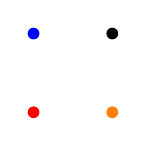
\begin{tikzpicture}[scale=1]
            \node (a) at (0,0) [circle,fill,inner sep=1.5pt,color=red] {};
            \node (b) at (0,1) [circle,fill,inner sep=1.5pt,color=blue] {};
            \node (c) at (1,0) [circle,fill=orange,inner sep=1.5pt] {};
            \node (d) at (1,1) [circle,fill,inner sep=1.5pt] {};

        \end{tikzpicture}
        \caption{\scriptsize Representación de una gráfica inconexa con 4 componentes.}
    \end{minipage}
    \hspace{0.015\textwidth}
    \begin{minipage}{0.2\textwidth}
        \centering
        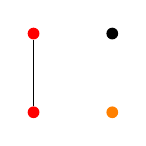
\begin{tikzpicture}[scale=1]
            \node (a) at (0,0) [circle,fill,inner sep=1.5pt,color=red] {};
            \node (b) at (0,1) [circle,fill,inner sep=1.5pt,color=red] {};
            \node (c) at (1,0) [circle,fill=orange,inner sep=1.5pt] {};
            \node (d) at (1,1) [circle,fill,inner sep=1.5pt] {};

            \draw (a) -- (b) ;

        \end{tikzpicture}
        \caption{\scriptsize Representación de una gráfica inconexa de 3 componentes.}
    \end{minipage}
    \hspace{0.015\textwidth}
    \begin{minipage}{0.2\textwidth}
        \centering
        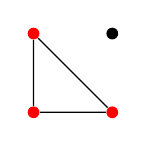
\begin{tikzpicture}[scale=1]
            \node (a) at (0,0) [circle,fill,inner sep=1.5pt,color=red] {};
            \node (b) at (0,1) [circle,fill,inner sep=1.5pt,color=red] {};
            \node (c) at (1,0) [circle,fill,inner sep=1.5pt,color=red] {};
            \node (d) at (1,1) [circle,fill,inner sep=1.5pt] {};


            \draw (a) -- (b) (a) -- (c) (b) -- (c);

        \end{tikzpicture}
        \caption{\scriptsize Representación de una gráfica inconexa de 2 componentes}
    \end{minipage}
    \hspace{0.015\textwidth}
    \begin{minipage}{0.2\textwidth}
        \centering
        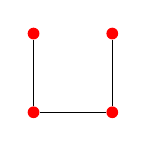
\begin{tikzpicture}[scale=1]
            \node (a) at (0,0) [circle,fill,inner sep=1.5pt,color=red] {};
            \node (b) at (0,1) [circle,fill,inner sep=1.5pt,color=red] {};
            \node (c) at (1,0) [circle,fill,inner sep=1.5pt,color=red] {};
            \node (d) at (1,1) [circle,fill,inner sep=1.5pt,color=red] {};

            \draw (a) -- (b) (a) -- (c) (d) -- (c) ;

        \end{tikzpicture}
        \caption{\scriptsize Representación de una gráfica conexa.}
    \end{minipage}
\end{figure}

\vspace{1cm}

%
% Ejercicio 5
%
\textbf{5}. Un \textit{hidrocarburo saturado} es una molécula $C_mH_n$ en la que cada átomo de carbono tiene cuatro enlaces, cada átomo de hidrógeno 
tiene un enlace y ninguna sucesión de enlaces forma un ciclo. Demuestre que para cualquier entero positvo $m$, la molécula $C_mH_n$ existe si y sólo si 
$n = 2m +2$.\\

Supongamos una secuancia $P$ \textit{(que es un camino)} de moléculas de Carbono de la sigueinte forma:

\begin{center}
    $P = (C_1, C_2, C_3, \dots,C_{m-1},C_m)$
\end{center}

Como sabemos que un átomo de Carbono tiene solamente $4$ enlaces y ademas no se forman ciclos en ninguna sucesion, entonces no podemos
tener un enlace entre ningun $C_i,C_j$ en $P$, con $i,j \in {1,2,3,\dots,m}$.\\

Como $C$ tiene $4$ enlaces, enlazaremos un $H$ a cada enlace libre de cada $C_i \in P$, de 
esta forma tendriamos que los átomos $(C_2, C_3,\dots,C_{m-1})$ tienen un enlace con $2$ átomos $H$, mientras los extremos $C_1$ y $C_m$ tendran enlace 
con $3$ átomos $H$. Es claro que para todos los átomos en la secuencia $P$ hay $2$ átomos $H$, $i.e$ $2m$, ademas para los extremos de la
misma tendremos $2$ átomos mas de $H$. así para $P$ con una cantidad $m$ de átomos de $C$, tendremos una cantidad $2m +2$ átomos de $H$.\\

Otro caso es cuando en lugar de enlazar un átomo $H$ a un enlace libre de algún $C_i$ enlazaramos una secuncias nueva $P' = (C'_1,C'_2, C'_3,\dots,C'_{k-1},C'_k)$ de átomos de $C$.
Como hemos quitado un átomo $H$ a dicho $C_i$, pero sabemos que toda la secuncia tendra en el extremo un átomo $C$ enlazado con 
$3$ átomos $H$ entonces podemos decir que no se altera la cantidad, pues $2m + 2$ es equivalente a  $2(m + k) +2$ elementos $H$ para una cantidad nueva $m + k$ de 
átomos $C$.\\

Por lo tanto, para cualquier cantidad $m$ de átomos $C_m$ un \textit{hidrocarburo saturado} es una molécula $C_mH_n$ donde $n = 2m +2$.$_{\blacksquare}$

\begin{figure}[h!]
    \centering
    \begin{minipage}{0.2\textwidth}
        \centering
        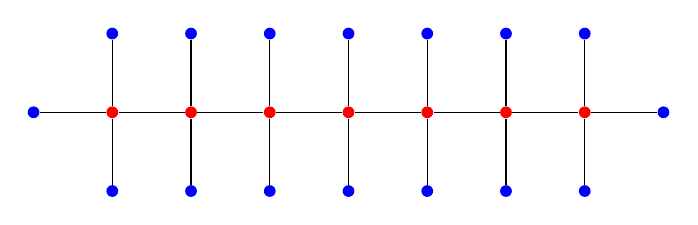
\begin{tikzpicture}[scale=1]
            \node (c1) at (0,0) [circle,fill,inner sep=1.5pt,color=red] {};
            \node (c2) at (1,0) [circle,fill,inner sep=1.5pt,color=red] {};
            \node (c3) at (2,0) [circle,fill,inner sep=1.5pt,color=red] {};
            \node (c4) at (3,0) [circle,fill,inner sep=1.5pt,color=red] {};
            \node (c5) at (4,0) [circle,fill,inner sep=1.5pt,color=red] {};
            \node (c6) at (5,0) [circle,fill,inner sep=1.5pt,color=red] {};
            \node (c7) at (6,0) [circle,fill,inner sep=1.5pt,color=red] {};

            \node (h1) at (-1,0) [circle,fill,inner sep=1.5pt,color=blue] {};
            \node (h2) at (0,-1) [circle,fill,inner sep=1.5pt,color=blue] {};
            \node (h3) at (0,1) [circle,fill,inner sep=1.5pt,color=blue] {};
            \node (h4) at (1,-1) [circle,fill,inner sep=1.5pt,color=blue] {};
            \node (h5) at (1,1) [circle,fill,inner sep=1.5pt,color=blue] {};
            \node (h6) at (2,-1) [circle,fill,inner sep=1.5pt,color=blue] {};
            \node (h7) at (2,1) [circle,fill,inner sep=1.5pt,color=blue] {};
            \node (h8) at (3,-1) [circle,fill,inner sep=1.5pt,color=blue] {};
            \node (h9) at (3,1) [circle,fill,inner sep=1.5pt,color=blue] {};
            \node (h10) at (4,-1) [circle,fill,inner sep=1.5pt,color=blue] {};
            \node (h11) at (4,1) [circle,fill,inner sep=1.5pt,color=blue] {};
            \node (h12) at (5,-1) [circle,fill,inner sep=1.5pt,color=blue] {};
            \node (h13) at (5,1) [circle,fill,inner sep=1.5pt,color=blue] {};
            \node (h14) at (6,-1) [circle,fill,inner sep=1.5pt,color=blue] {};
            \node (h15) at (6,1) [circle,fill,inner sep=1.5pt,color=blue] {};
            \node (h16) at (7,0) [circle,fill,inner sep=1.5pt,color=blue] {};

            \draw (h1) --(c1) -- (c2) -- (c3) -- (c4) -- (c5) -- (c6) -- (c7) -- (h16)  
            (h3) -- (c1) -- (h2)  (h5) -- (c2) -- (h4)  (h7) -- (c3) -- (h6)
            (h9) -- (c4) -- (h8)  (h11) -- (c5) -- (h10)  (h13) -- (c6) -- (h12)  (h15) -- (c7) -- (h14);

        \end{tikzpicture}
        \caption{\scriptsize Gráfica que representa un enlace $C_mH_n$.}
    \end{minipage}
\end{figure}


\vspace{1cm}

%
% Ejercicio 6
%
\textbf{6}. Demuestre que una suseción $(d_1,...,d_n)$ de enteros positivos es la suseción de grados de un árbol si
y sólo si $\sum_{i=1}^{n} d_i = 2(n-1)$.\\

{\color{blue} [$\Rightarrow]$} Una suseción $(d_1,...,d_n)$ de enteros positivos es la suseción de grados de un árbol\\

Por construcción de un árbol, analizando la suseción de grados para una gráfica arbitraria $|V_G| = n$, recordemos que 
la forma en cómo sabemos el grado de un vértice es por las aristas que indicen en el, y sabiendo que el número de aristas 
de un árbol esta dado por $|E| = |V|-1$. Entonces la suma de sus grados esta dada por $n-1$.\\

Sin embargo, recordemos que el papel de una arista, es hacer a dos vértices adyacentes. Por lo que si solo sumamos el número 
de aristas de una gráfica, en realidad, solo estaríamos sumando la mitad de grados de un árbol arbitrario. Por lo que, 
para una suseción $(d_1,...,d_n)$, la suma de los grados de estos vertices esta dado de la forma: 

\[
\sum_{i=1}^{n} d_i = 2(n-1)
\]

\vspace{1cm}


{\color{blue} [$\Leftarrow]$} Sea una suma $\sum_{i=1}^{n} d_i = 2(n-1)$ de grados de una gráfica $G$\\

Sabiendo que la suma que tenemos representa a los grados de una gráfica que, por construcción, esta dada por su número de 
aristas. Se infiere que se trata de un árbol, pues su número de aristas esta dado por $|E| = |V|-1$.\\

Por hipótesis, en la suma dada podemos inferir que $d_i$ representa el grado que tiene un vertice arbitrario, por lo que 
podemos suponer que tenemos una suseción del tipo $(d_1,...,d_n)$. Por lo que resta demostrar que la suseción es de enteros 
positivos con inducción.\\

\textbf{Caso Base}: Tenemos $|V| = n =  2$, por lo que la suma esta dada por $\sum_{i=1}^{1} d_1 = 2(n-1)$, lo que nos 
da que $2(2-1) = 2$ y entonces nos queda la suseción: $(1, 1)$. La cual sí cumple que con ser un árbol de dos vertices, 
pues cada vertice tendría grado 1.\\

\textbf{Hipótesis de inducción:} Supongamos que para todo $k$ tal que $2 \le k < n$, toda sucesión de enteros 
positivos $(d_1,\dots,d_k)$ satisface
\[
\sum_{i=1}^k d_i = 2(k-1)
\]
que es la secuencia de grados de algún árbol con $k$ vértices.\\

\textbf{Paso inductivo: } Suponiendo que se cumple para k - 1: 

\[
\sum_{i=1}^{k-1} d_i = 2(k-1).
\]

Esto debido al deducir que podemos volver a nuestro caso base, eliminando una hoja, a la vez, de nuestra suseción. Digamos que $v_1$ 
es esa hoja en nuestra suseción con grado 1, tal que nos quedaría: $(d_2,\dots,d_k)$ y como $v_1$ estaba conectado a otro vertice, 
digamos $v_f$, entonces este vertice va a tender a convertirse en una rama con dos hojas o una hoja, tal que $(d_2,\dots,d_f - 1,\dots,d_k)$.\\

En cualquier caso, la suma nos quedaría como sigue: 

\[
\sum_{i=2}^k d_i - 1 = \left(\sum_{i=1}^k d_i\right) - 2 = 2(k-1) - 2 = 2\bigl((k-1)-1\bigr).
\]


Notese que primero hacemos la suma quitando el vertice $v_1$, luego le restamos dos porque es el número de incidencias 
que hacía dicho vertice en nuestra suma, y por último obtenemos una subgráfica de nuestro árbol original. La cual, es la que queríamos.\\ 

Esto a la larga nos va llevar a nuestro caso base, por lo que al final, si reicorporamos el vertice que 
habíamos quitado, tendríamos que $v_1v_f \in E_G$. Lo que nos dice que, en realidad, la suma con la que hemos estado 
trabajando se trata de una suseción $(d_1,\dots,d_f,\dots,d_n)$ de enteros positivos de grados de un árbol
\hfill $\Box$


\vspace{1cm}

%
% Ejercicio Extra 3
%
\textbf{Extra 3}. Sea $\mathcal{T}$ una familia de subárboles de un árbol $T$. Demuestre que si cualesquiera dos elementos de $\mathcal{T}$
tienen un vértice en común, enotnces hay un vértice de $T$ que está en todos los elementos de $T$.

\begin{tcolorbox}[title=\textbf{Hipotesis}, colback=red!15!white, colframe=black!, breakable]
	$\mathcal{T}$ es una familia de subárboles de $T$.\\

    $T$ es un árbol, entonces sabemos que $T$ es conexa y ademas cada arista de $T$ es un puente.
\end{tcolorbox}

Como $T$ es un árbol, entonces hay un camino entre cualesquiera dos vértices $t_m,t_n \in T$ y ademas sabemos que esta trayectoria es única, si
no fuera así, $T$ tendría un ciclo. Así, pensemos en dos subarboles $\mathcal{R}$ y $\mathcal{S}$ en $T$ tal que existe una trayectoria
entre cualesquiera vértices $r_m,r_n \in \mathcal{R}$ y $s_m,s_n \in \mathcal{S}$\\

Sabemos que $\mathcal{S}$ y $\mathcal{R}$ no pueden contener ciclos pues $T$ no los contiene. De esta forma debe existir un vértice 
$r_i$ y $s_i$ que cumplan $r_i = s_i$, de no ser así entonces aseguramos que $\nexists$ un camino $(r_0,s_0), (r_0,s_m), (r_m,s_0)$ y $(r_m,s_m)$, como esto no puede ser
pues $T$ es conexa, entonces existe un vértice $r_i$ de $\mathcal{R}$ y un vértice $s_i$ de $\mathcal{S}$ que deben ser iguales, así para cualesqueira $\mathcal{T}, \mathcal{T}'$ de $T$
existe un vértice $t_i$ que pertece a $T$ tal que pertenece a cualquier $\mathcal{T}$ subárbol de $T$ que nos garantiza la conexidad de $T$.$_{\blacksquare}$



\end{document}
